\documentclass[aspectratio=169]{../latex_main/tntbeamer}  % you can pass all options of the beamer class, e.g., 'handout' or 'aspectratio=43'
\usepackage{dsfont}
\usepackage{bm}
\usepackage[english]{babel}
\usepackage[T1]{fontenc}
%\usepackage[utf8]{inputenc}
\usepackage{graphicx}
\graphicspath{ {./figures/} }
\usepackage{algorithm}
\usepackage[ruled,vlined,algo2e,linesnumbered]{algorithm2e}
\usepackage{hyperref}
\usepackage{booktabs}
\usepackage{mathtools}

\usepackage{amsmath,amssymb}

\DeclareMathOperator*{\argmax}{arg\,max}
\DeclareMathOperator*{\argmin}{arg\,min}

\usepackage{amsbsy}
\newcommand{\vect}[1]{\bm{#1}}
%\newcommand{\vect}[1]{\boldsymbol{#1}}

\usepackage{pgfplots}
\pgfplotsset{compat=1.16}
\usepackage{tikz}
\usetikzlibrary{trees} 
\usetikzlibrary{shapes.geometric}
\usetikzlibrary{positioning,shapes,shadows,arrows,calc,mindmap}
\usetikzlibrary{positioning,fadings,through}
\usetikzlibrary{decorations.pathreplacing}
\usetikzlibrary{intersections}
\pgfdeclarelayer{background}
\pgfdeclarelayer{foreground}
\pgfsetlayers{background,main,foreground}
\tikzstyle{activity}=[rectangle, draw=black, rounded corners, text centered, text width=8em]
\tikzstyle{data}=[rectangle, draw=black, text centered, text width=8em]
\tikzstyle{myarrow}=[->, thick, draw=black]

% Define the layers to draw the diagram
\pgfdeclarelayer{background}
\pgfdeclarelayer{foreground}
\pgfsetlayers{background,main,foreground}

% Requires XeLaTeX or LuaLaTeX
%\usepackage{unicode-math}

\usepackage{fontspec}
%\setsansfont{Arial}
\setsansfont{RotisSansSerifStd}[ 
Path=../latex_main/fonts/,
Extension = .otf,
UprightFont = *-Regular,  % or *-Light
BoldFont = *-ExtraBold,  % or *-Bold
ItalicFont = *-Italic
]
\setmonofont{Cascadia Mono}[
Scale=0.8
]

% scale factor adapted; mathrm font added (Benjamin Spitschan @TNT, 2021-06-01)
%\setmathfont[Scale=1.05]{Libertinus Math}
%\setmathrm[Scale=1.05]{Libertinus Math}

% other available math fonts are (not exhaustive)
% Latin Modern Math
% XITS Math
% Libertinus Math
% Asana Math
% Fira Math
% TeX Gyre Pagella Math
% TeX Gyre Bonum Math
% TeX Gyre Schola Math
% TeX Gyre Termes Math

% Literature References
\newcommand{\lit}[2]{\href{#2}{\footnotesize\color{black!60}[#1]}}

%%% Beamer Customization
%----------------------------------------------------------------------
% (Don't) Show sections in frame header. Options: 'sections', 'sections light', empty
\setbeamertemplate{headline}{empty}

% Add header logo for normal frames
\setheaderimage{
	% 
\includegraphics[height=\logoheight]{figures/TNT_darkv4.pdf}
	
\includegraphics[height=\logoheight]{../latex_main/figures/luh_logo_rgb_0_80_155.pdf}
	% 
\includegraphics[height=\logoheight]{figures/logo_tntluh.pdf}
}

% Header logo for title page
\settitleheaderimage{
	% 
\includegraphics[height=\logoheight]{figures/TNT_darkv4.pdf}
	
\includegraphics[height=\logoheight]{../latex_main/figures/luh_logo_rgb_0_80_155.pdf}
	% 
\includegraphics[height=\logoheight]{figures/logo_tntluh.pdf}
}

% Title page: tntdefault 
\setbeamertemplate{title page}[tntdefault]  % or luhstyle
% Add optional title image here
%\addtitlepageimagedefault{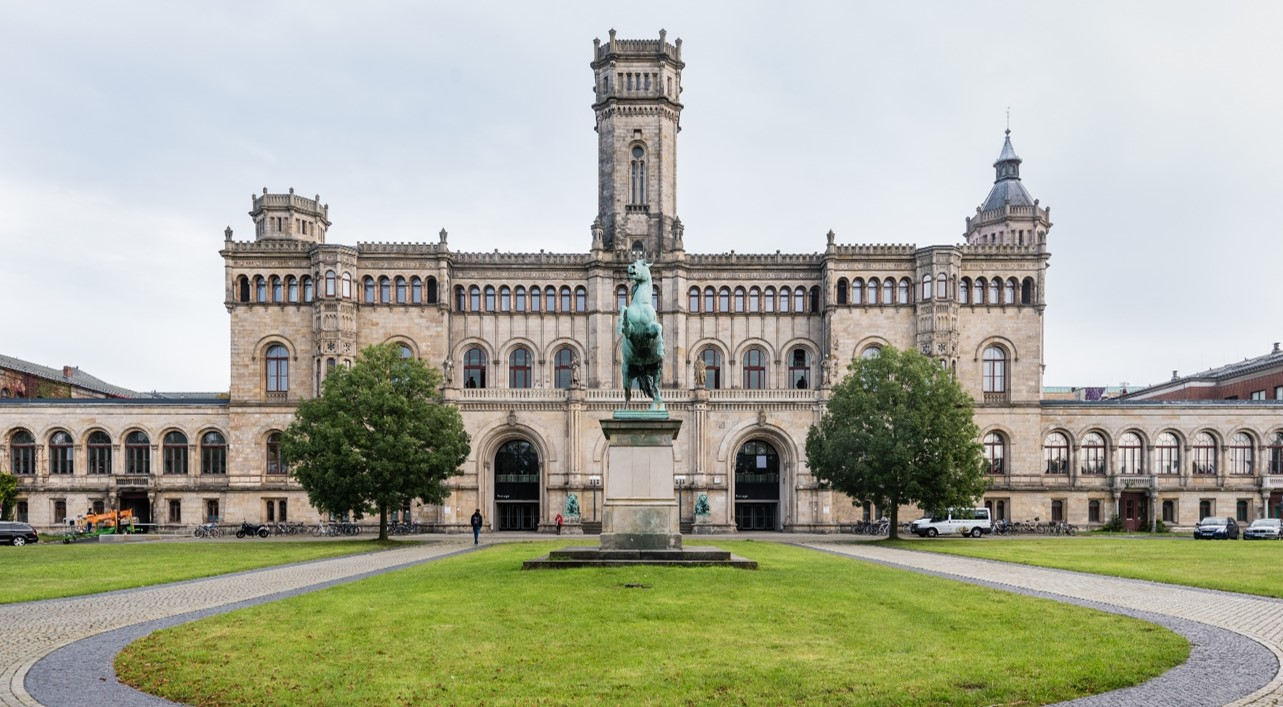
\includegraphics[width=0.65\textwidth]{figures/luh_default_presentation_title_image.jpg}}

% Title page: luhstyle
% \setbeamertemplate{title page}[luhstyle]
% % Add optional title image here
% \addtitlepageimage{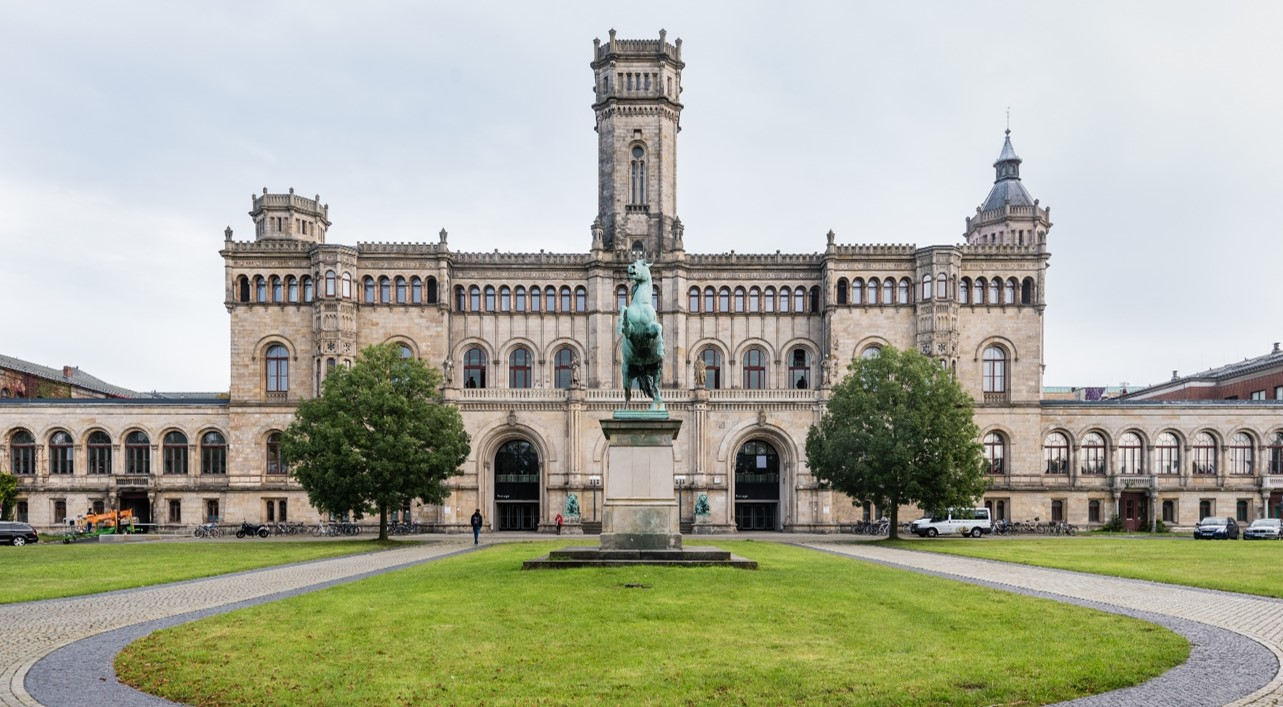
\includegraphics[width=0.75\textwidth]{figures/luh_default_presentation_title_image.jpg}}

\author[Abedjan \& Lindauer]{Ziawasch Abedjan \& Marius Lindauer\\[1em]
	
\includegraphics[height=\logoheight]{../latex_main/figures/luh_logo_rgb_0_80_155.pdf}\qquad
	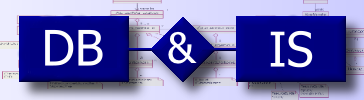
\includegraphics[height=\logoheight]{../latex_main/figures/DBIS_Kurzlogo.png}\qquad

\includegraphics[height=\logoheight]{../latex_main/figures/TNT_darkv4}\qquad

\includegraphics[height=\logoheight]{../latex_main/figures/L3S.jpg}	}
\date{Summer Term 2022; \hspace{0.5em} {
\includegraphics[height=1.5em]{../latex_main/figures/Cc-by-nc-sa_icon.svg.png}}; based on \href{https://ds100.org/fa21/}{[DS100]}
}


%%% Custom Packages
%----------------------------------------------------------------------
% Create dummy content
\usepackage{blindtext}

% Adds a frame with the current page layout. Just call \layout inside of a frame.
\usepackage{layout}


%%% Macros
%\renewcommand{\vec}[1]{\mathbf{#1}}
% \usepackage{bm}
%\let\vecb\bm

\title[Introduction]{DS: Data Sampling and Probability}
\subtitle{Bias}

\graphicspath{ {./figure/} }
%\institute{}


\begin{document}
	
	\maketitle
	\begin{frame}{Case study – 1936 Presidential Election}
	  \begin{figure}
	      \centering
	      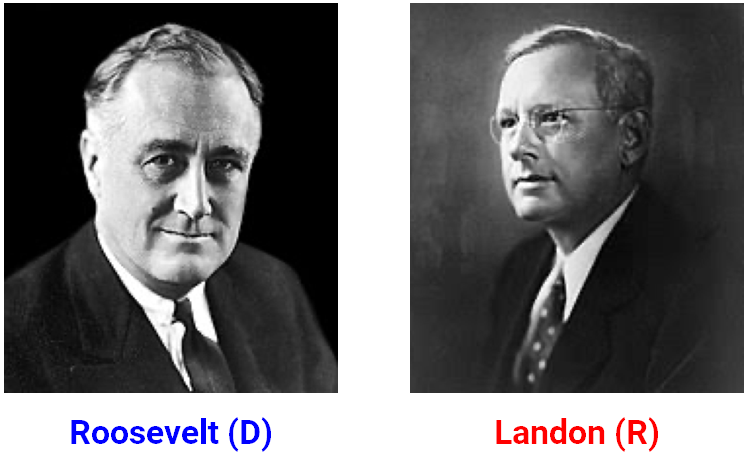
\includegraphics[scale=.4]{Bild11}
	  \end{figure}
	  In 1936, President Franklin D. Roosevelt (left) went up for re-election against Alf Landon (right). As is usual, polls were conducted in the months leading up to the election to try and predict the outcome.

	\end{frame}
	
	\begin{frame}{The Literary Digest}
	    \begin{columns}
	        \begin{column}{.4\textwidth}
	            The Literary Digest was a magazine. They had successfully predicted the outcome of 5 general elections coming into 1936.
	            \bigskip
	            
	            They sent out their survey to 10,000,000 individuals, who they found from:
	            \begin{itemize}
	                \item Phone books.
	                \item Lists of magazine subscribers.
	                \item Lists of country club members.
	            \end{itemize}
	        \end{column}
	        
	        \begin{column}{.5\textwidth}
	            \begin{figure}
	                \centering
	                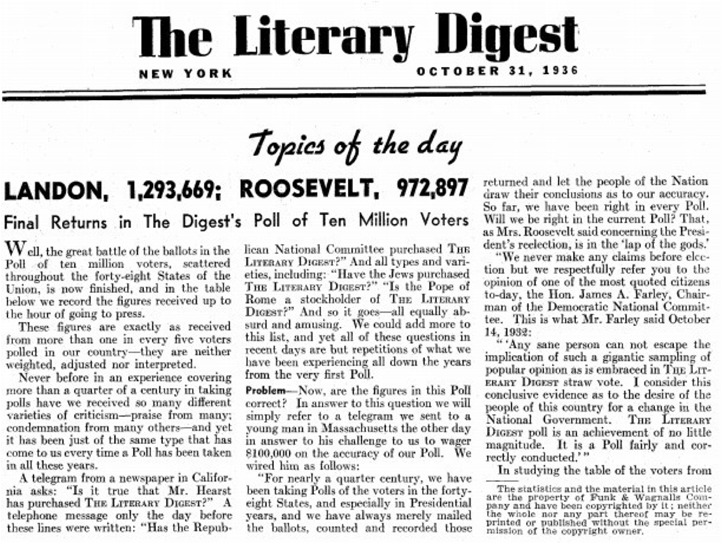
\includegraphics[scale=.58]{Bild12}
	            \end{figure}
	        \end{column}
	        
	    \end{columns}
	    
	\end{frame}
	
	
	\begin{frame}{The Literary Digest}
	    \begin{columns}
	        \begin{column}{.4\textwidth}
	            \bigskip


	            The Literary Digest’s prediction:
                \begin{align*}
                    \text{43\% Roosevelt, 57\% Landon}
                \end{align*}
                The actual outcome of the election:
                \begin{align*}
                    \text{61\% Roosevelt, 37\% Landon}
                \end{align*}
                How could this have happened? They surveyed 10 million people!
	        \end{column}
	        
	        \begin{column}{.5\textwidth}
	            \begin{itemize}
	                \item Their sample was not representative of the population.
	                \begin{itemize}
	                    \item They sampled people who owned phones, subscribed to magazines, and went to country clubs, who at the time were more affluent.
	                    \item These people tended to vote Republican (Alf Landon).
	                \end{itemize}
	                \item Only 2.4 million people actually filled out the survey!
	                \begin{itemize}
	                    \item 24\% response rate (low).
	                    \item Who knows how the other 76\% would have polled?
	                \end{itemize}
	            \end{itemize}
	        \end{column}
	        
	    \end{columns}
	    
	\end{frame}
	
	\begin{frame}{Gallup’s Poll}
	    \begin{columns}
	        \begin{column}{.4\textwidth}
	            George Gallup, a rising statistician, also made predictions about the impending 1936 elections. He predicted that Roosevelt would win with 56\% of the vote.
                \bigskip
                Not only was his estimate much closer than The Literary Digest’s estimate, but he did it with a sample size of only 50,000!
	        \end{column}
	        
	        \begin{column}{.5\textwidth}
	            George Gallup also predicted what The Literary Digest was going to predict, within 1\%. How was he able to predict what they were going to predict, with such accuracy?
                
                \begin{itemize}
                    \item He predicted that they would survey people in the phone book, people who subscribed to magazines, and who were part of country clubs.
                    \item So he sampled those same individuals!
                    \item He was able to predict their prediction by sampling only 3000 people.
                \end{itemize}
	        \end{column}
	        
	    \end{columns}
	    
	\end{frame}
	
	\begin{frame}{Summary of results}
	    \begin{columns}
	        \begin{column}{.6\textwidth}
	            \begin{tabular}{|l|l|l|}
	                \hline
	                 & \% Roosevelt & \#surveyed  \\
	               \hline
	               The Literary Digest poll  & 43\%  & 10,000,000\\
	               \hline
	               George Gallup’s poll & 56\% & 50,000\\
	               \hline
	               George Gallup’s\\ prediction of\\ Digest’s prediction & 44\% & 3,000\\
	               \hline
	               Actual election & 61\% & All voters\\
	               \hline
	            \end{tabular}
	        \end{column}
	        
	        \begin{column}{.4\textwidth}
	            Big samples aren’t always good!
                \begin{itemize}
                    \item What you need is a representative sample. 
                    \item If your sampling method is biased, those biases will be magnified with a larger sample size.
                \end{itemize}
	        \end{column}
	        
	    \end{columns}
	    
	\end{frame}
	
	
		\begin{frame}{Population, samples, and sampling frame}
	    \begin{columns}
	        \begin{column}{.4\textwidth}
	            \begin{itemize}
	                \item Population: The group that you want to learn something about.
                    \item Sampling Frame: The list from which the sample is drawn.
                    \begin{itemize}
                        \item If you’re sampling people, the sampling frame is the set of all people that could possibly end up in your sample.
                    \end{itemize}
                    \item Sample: Who you actually end up sampling. 
                    \begin{itemize}
                        \item A subset of your sampling frame.
                    \end{itemize}
	            \end{itemize}
	        \end{column}
	        
	        \begin{column}{.4\textwidth}
                \begin{figure}
                    \centering
                    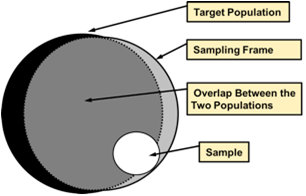
\includegraphics[scale=.5]{Bild13}\\
                    Note: There may be individuals in your sampling frame (and hence, your sample) that are not in your population!

                \end{figure}
	        \end{column}
	        
	    \end{columns}
	    
	\end{frame}
	
	
	\begin{frame}{Common Biases}
	    Selection Bias
        \begin{itemize}
            \item Systematically excluding (or favoring) particular groups.
            \item How to avoid: Examine the sampling frame and the method of sampling.
        \end{itemize}
        Response Bias
        \begin{itemize}
            \item People don’t always respond truthfully.
            \item How to avoid: Examine the nature of questions and the method of surveying.
        \end{itemize}
        Non-response Bias
        \begin{itemize}
            \item People don’t always respond.
            \item How to avoid: Keep your surveys short, and be persistent.
            \item People who don’t respond aren’t like the people who do!
        \end{itemize}
	\end{frame}
	
\end{document}